\documentclass[a4paper,10pt]{article}
\usepackage[utf8]{inputenc}
\usepackage[MeX]{polski}
\usepackage{graphicx}

\title{[MBI.A] Asembler DNA, sparowane końce - dokumentacja końcowa}
\author{Michał Aniserowicz, Jakub Turek}
\date{}

\begin{document}

\maketitle

\section*{Opis problemu}

Zadanie polega na implementacji aplikacji, która umożliwia tworzenie \emph{scaffoldów} na podstawie dostarczonych zbiorów \emph{contigów} oraz sekwencji PET. 

\begin{center}
  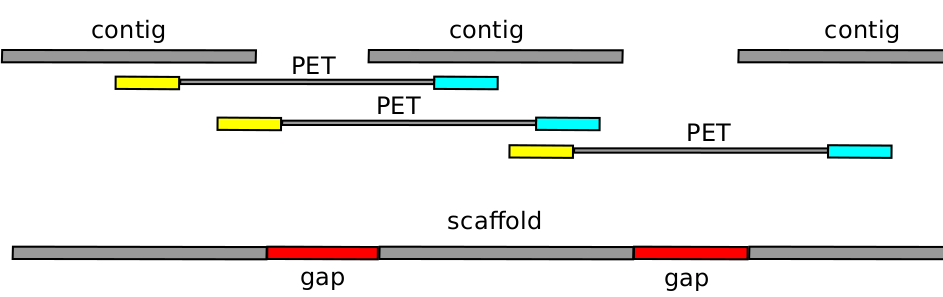
\includegraphics[width=.9\textwidth]{contig_pet.png}
\end{center}

\section*{Założenia}

W~ogólnym przypadku rekonstrukcja sekwencji \emph{contigów} nie jest możliwa. Z~tego względu, na potrzeby projektu przyjęto następujące założenia:

\begin{itemize}
  \item Początki i~końce łańcuchów PET to sekwencje unikalne. Wystąpienie takiej sekwencji w~jednym z~\emph{contigów} oznacza, że jest to odpowiednio początek lub koniec sekwencji PET.
  \item Badane są wyłącznie takie permutacje \emph{contigów}, dla których wystąpienie początku sekwencji PET implikuje przynajmniej częściowe wystąpienie jej końca w~dalszej części łańcucha. Innymi słowy początek lub koniec sekwencji PET nie może w~całości wystąpić w~przerwie (\emph{gap}) \emph{scaffoldu}.
  
    \begin{itemize}
	  \item Wyjątkiem od tej reguły jest początek i~koniec \emph{scaffoldu}, gdzie mogą występować, odpowiednio, niesparowane końce lub początki sekwencji PET.
    \end{itemize}
  
  \item Sekwencje należące do różnych par sparowanych końców mogą częściowo zachodzić na siebie.
\end{itemize}

\section*{Algorytm}

Do rozwiązania zadania użyty został algorytm typu brute-force działający na wstępnie odfiltrowanym zbiorze kombinacji contigów.
Algorytm przebiega według następującego schematu:

\begin{enumerate}
 \item \label{step1} Wyznaczane są wszystkie permutacje zadanego zbioru \emph{contigów}.
 \item \label{step2} Permutacje zostają wstępnie sprawdzone:
  \begin{itemize}
   \item następuje próba znalezienia sekwecji PET, której początek i koniec w całości zawiera się w dowolnej parze \emph{contigów}:
    \begin{itemize}
     \item jeśli taka sekwencja nie zostanie znaleziona, wszyskie permutacje zostają uwzględnione w kolejnych krokach algorytmu;
    \end{itemize}
   \item każda permutacja jest sprawdzana pod względem kolejności wystąpienia \emph{contigów} zawierających znalezioną sekwencję:
    \begin{itemize}
     \item jeśli \emph{contig} zawierający początek sekwencji znajduje się przed \emph{contigiem} zawierającym jej koniec, to dana permutacja zostaje uwzględniona w kolejnych krokach algorytmu,
     \item w przeciwnym wypadku, permutacja zostaje odrzucona.
    \end{itemize}
  \end{itemize}
 \item \label{step3} Na podstawie każdej z zaakceptowanych permutacji budowany jest \emph{scaffold}:
  \begin{itemize}
   \item dla każdej sekwencji PET:
    \begin{enumerate}
     \item \label{step3_1} następuje próba znalezienia \emph{contiga} zawierającego (w całości lub częściowo\footnote{Częściowe pokrycie sekwencji PET występuje, gdy \emph{contig} zaczyna się końcem fragmentu (tzn. początku lub końca) danej sekwencji lub kończy początkiem fragmentu tej sekwecji. Minimalny akceptowalny stosunek części pokrytej do całości fragmentu określony jest w pliku konfiguracyjnym aplikacji.}) początek sekwencji,
     \item \label{step3_2} przeglądane są \emph{contigi} występujące po znalezionym, w celu odnalezienia \emph{contiga} zawierającego koniec sekwecji,
     \item \label{step3_3} jeśli odległość pomiędzy znalezioną parą \emph{conitgów} dopuszcza istnienie pomiędzy nimi sekwencji PET, to  pomiędzy te \emph{contigi} wstawiany jest odpowiedniej długości \emph{gap},
     \item \label{step3_4} jeśli w którymkolwiek z powyższych kroków nastąpiło niepowodzenie (odpowiedni \emph{conitg} nie został odnaleziony lub sprawdzenie odległości dało wynik negatywny), to wykonywane jest sprawdzenie, czy pierwszy \emph{contig} zawiera koniec sekwecji lub czy ostatni \emph{conitg} zawiera jej  początek - taka sytuacja uznawana jest za poprawną,
     \item \label{step3_5} aktualizowany jest ranking \emph{R}, określający liczbę pokrywających się zasad początku lub końca sekwencji PET z odnalezionymi \emph{contigami}.
    \end{enumerate}
   \item jeżeli \emph{R} $> 0$, to dany \emph{scaffold} dodawany jest listy wynikowej algorytmu.
  \end{itemize}
 \item \label{step4} Uzyskana lista \emph{scaffoldów} sortowana jest według malejących wartości \emph{R}.
\end{enumerate}

\section*{Implementacja}

Projekt został zaimplementowany w~języku C\# (platforma .NET). Testy jednostkowe zostały napisane w~oparciu o~platformę NUnit\footnote{http://www.nunit.org/}, z~użyciem biblioteki Rhino Mocks\footnote{http://www.ayende.com/wiki/Rhino+Mocks.ashx}.

Aplikacja posiada interfejs okienkowy stworzony w~technologii WPF, umożliwiający odczyt danych wejściowych z/zapis danych wyjściowych do pliku. Na dane wejściowe składają się:

\begin{itemize}
 \item Opis \emph{conitgów} w~postaci łańcuchów tekstowych oddzielonych znakami nowej linii.
 
  \begin{verbatim}
    ACAGCTTA
    CCGGGTAC
    TACAGCTT
  \end{verbatim}
  \item Opis sekwencji PET w~postaci dwóch sekwencji (początek, koniec) oraz długości łańcucha. Dane w~sekwencji oddzielone przecinkami, natomiast kolejne PET'y oddzielone znakami nowej linii.
  
  \begin{verbatim}
   GATC,CCAT,100
   GGCT,AGAA,1500
  \end{verbatim}
\end{itemize}

Dane wyjściowe to uporządkowana sekwencja \emph{contigów} oddzielonych znakami spacji reprezentującymi długość przerwy (\emph{gap}).

  \begin{verbatim}
   CCGGGTAC       TACAGCTT  ACAGCTTA
  \end{verbatim}

\section*{Przykład}

\begin{itemize}
 \item Plik wejściowy:
  \begin{verbatim}
   ACAGCTTA
   CCGGGTAC
   TACAGCAA

   CCG,TACA,15
   GCA,GCT,13
  \end{verbatim}
 \item Plik wyjściowy:
  \begin{verbatim}
   CCGGGTAC   TACAGCAA   ACAGCTTA
  \end{verbatim}
\end{itemize}

\section*{Testowanie}
Program wykonany w ramach projektu tworzony był z wykorzystaniem metodyki Test Driven Development\footnote{http://pl.wikipedia.org/wiki/Test-driven\_development}, czego skutkiem jest znaczne pokrycie testami jednostkowymi - testów jest ok. 70. Przetestowane zostały m.in. następujące przypadki:
\begin{itemize}
 \item odrzucenie niepoprawnych permutacji \emph{contigów} (patrz krok \ref{step2} algorytmu),
 \item odnalezienie całkowitego pokrycia fragmentów sekwencji PET przez sąsiadujące \emph{contigi} (kroki \ref{step3_1}, \ref{step3_2}),
 \item odnalezienie całkowitego pokrycie fragmentów sekwencji PET przez \emph{contigi} oddalone od siebie (kroki \ref{step3_1}, \ref{step3_2}),
 \item odnalezienie wystąpienia końca fragmentu sekwencji PET w początku \emph{contigu} (krok \ref{step3_1} / \ref{step3_2}),
 \item odnalezienie wystąpienia początku fragmentu sekwencji PET w końcu \emph{contigu} (krok \ref{step3_1} / \ref{step3_2}),
 \item odnalezienie całkowitego pokrycia pomimo występującego we wcześniejszym \emph{contigu} pokrycia częściowego (kroki \ref{step3_1} / \ref{step3_2}),
 \item wstawienie \emph{gapów} pomiędzy dwa \emph{contigi} całkowicie pokrywające fragmenty sekwencji PET (krok \ref{step3_3}),
 \item wstawienie \emph{gapów} pomiędzy dwa \emph{contigi} częściowo pokrywające fragmenty sekwencji PET (krok \ref{step3_3}),
 \item weryfikacja odległości pomiędzy \emph{conitgami} (krok \ref{step3_3}),
 \item odnalezienie niesparowanego końca sekwencji PET w pierszym \emph{contigu} (krok \ref{step3_4}),
 \item odnalezienie niesparowanego początku sekwencji PET w ostatnim \emph{contigu} (krok \ref{step3_4}),
 \item obliczanie rankingu \emph{R} \emph{scaffoldu} (krok \ref{step3_5}),
 \item odrzucenie \emph{scaffoldów} o zerowej wartości rankingu \emph{R} (krok \ref{step3}),
 \item sortowanie \emph{scaffoldów} według wartości rankingu \emph{R} (krok \ref{step4}).
\end{itemize}

Ponadto dokonano wielokrotnych ``ręcznych'' testów z wykorzystaniem przygotowanych danych wejściowych. Wynik wszystkich testów był pozytywny.

\section*{Wnioski}

Proces budowania poprawnego \emph{scaffoldu} wydaje się być prostą i wydajną sekwencją operacji na ciągach znaków.
Biorąc jendak pod uwagę ilość kombinacji, które należy sprawdzić ($n!$, gdzie $n$ to liczność zadanego zbioru \emph{contigów}), nie dziwi fakt, że algorytmy tego typu
są wymagające zarówno pamięciowo jak i obliczeniowo.

Potencjalnym usprawnieniem działania algorytmu może być zastosowanie lepszej heurystyki podczas wstępnego filtrowania kombinacji \emph{contigów}.
Obecna implementacja odrzuca tylko około połowę kombinacji, co dla zestawu dziesięciu \emph{conitgów} pozostawia do dalszego przetworzenia ok. 1,8 mln kombinacji.

\end{document}